\documentclass[aspectratio=169]{beamer}
\usetheme{Madrid}

\usepackage{graphicx}
\usepackage[utf8]{inputenc}
\usepackage{hyperref}
\usepackage{listings}
\usepackage{xcolor}

%\decimalpoint

\begin{document}

\title{Introduction to Neural Networks}  
\subtitle{Application to classification} 
\author[J.I. Vasquez]{\textbf{Juan Irving Vásquez} \\jivg.org}
\date{\today \copyright}
\institute[jivg.org]{Centro de Innovación y Desarrollo Tecnológico en Cómputo \\ Instituto Politécnico Nacional}
% logo of my university
\titlegraphic{
\includegraphics[width=2cm]{ipn-cidetec}}
\frame{\titlepage} 

\frame{
	\frametitle{Contents}
	\tableofcontents
}

\AtBeginSection[] { \begin{frame} \frametitle{Roadmap} \tableofcontents[currentsection] \end{frame} }



%%%%%%%%%%%%%%%%%%%%%%%%%%%%%%%%%%%%%%%%%%%%%%%%%%%%%%%%



\section{Classification}


\frame{
	\frametitle{Classification}
	\begin{itemize}
		\item It consist on assigning classes or labels to objects [Sucar 15].
		\begin{center}
		
\includegraphics[width=0.7\linewidth]{./banner_animal_classifications}
		\end{center}
	\end{itemize}
}


\frame{
\frametitle{Classification (2)}
\begin{description}
\item [Unsupervised] In this case the classes are unknown. The problem consists in dividing a set of objects into $n$ groups or clusters, so that a class is assigned to each different group. Clustering.
\item [Supervised] The possible classes or labels are known a priori, and the problem consists in finding a function or rule that assigns each object to one of the classes.
\end{description}

\begin{block}{Target task}
	Feed forward networks (multilayer perceptrons) can only deal with supervised learning
\end{block}
}


\frame{
\frametitle{Supervised Classification}
\begin{center}

\begin{figure}
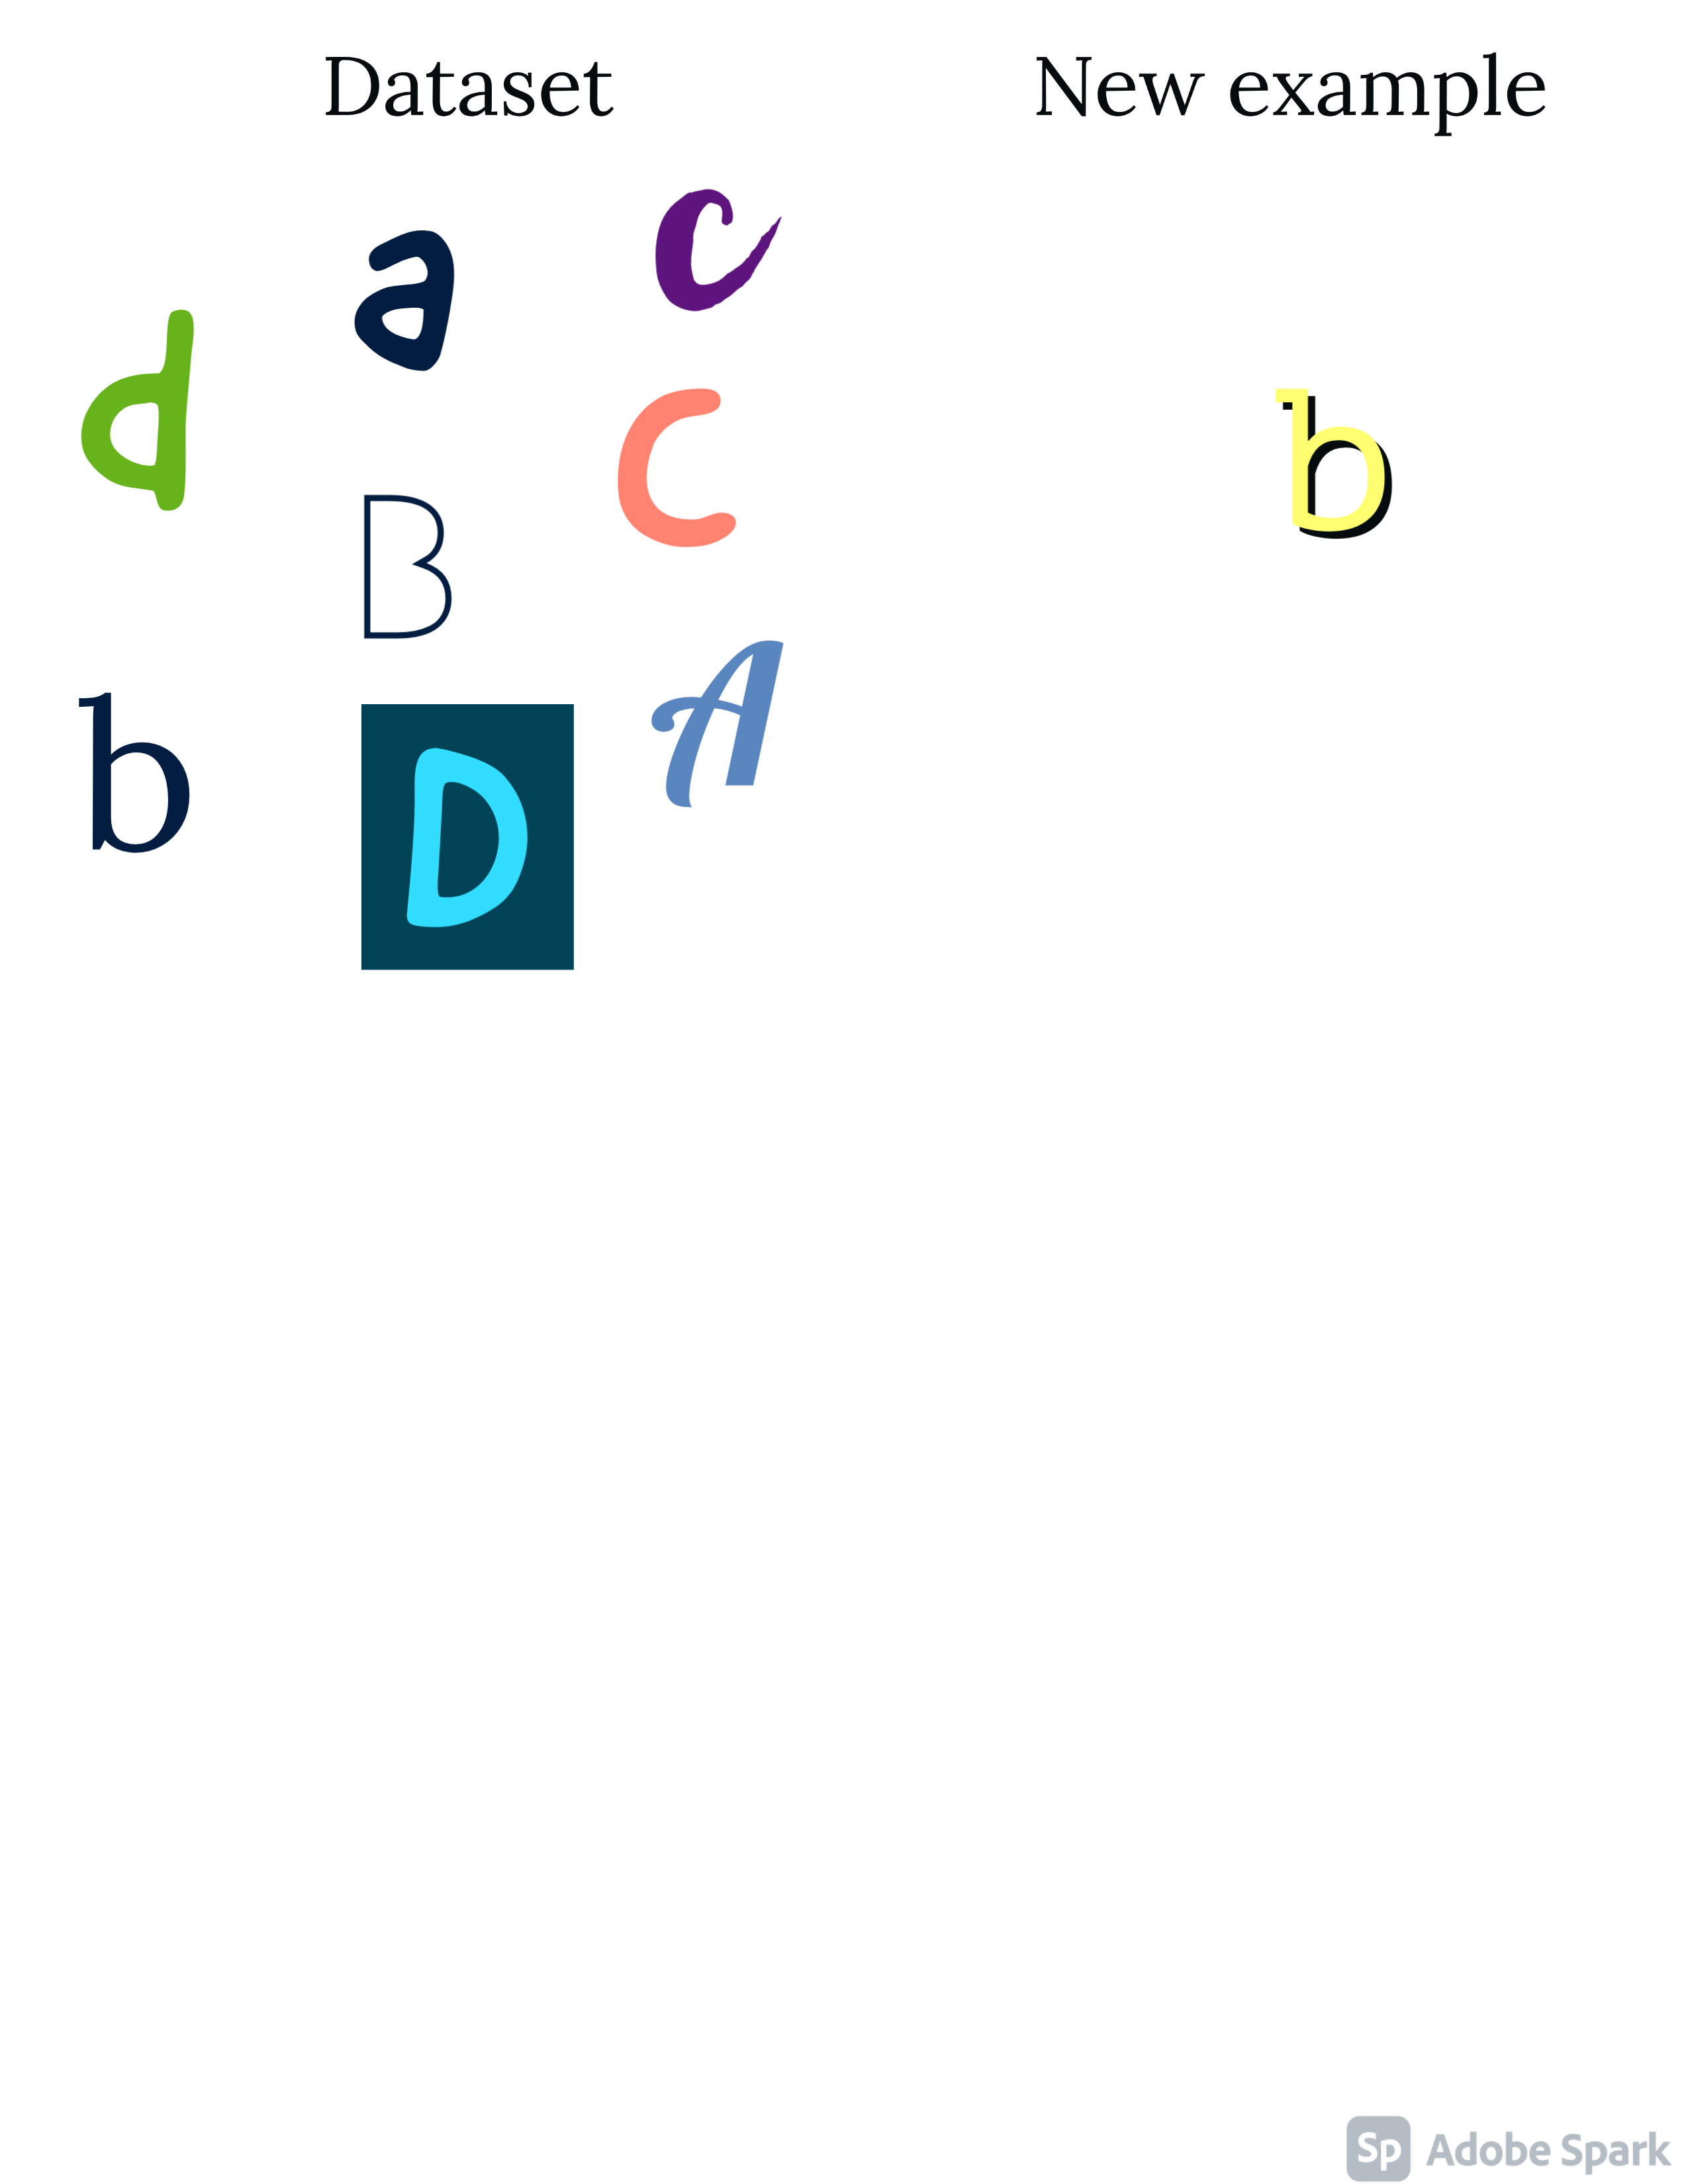
\includegraphics[trim={0 3cm 0 3cm},clip,height=0.8\linewidth]{./classification}\footnote{The new example }
\caption{What is the class of the new example?}
\end{figure}
\end{center}
}



%\frame{
%	\frametitle{One-hot encoding - quiz}
%	\begin{center}
%		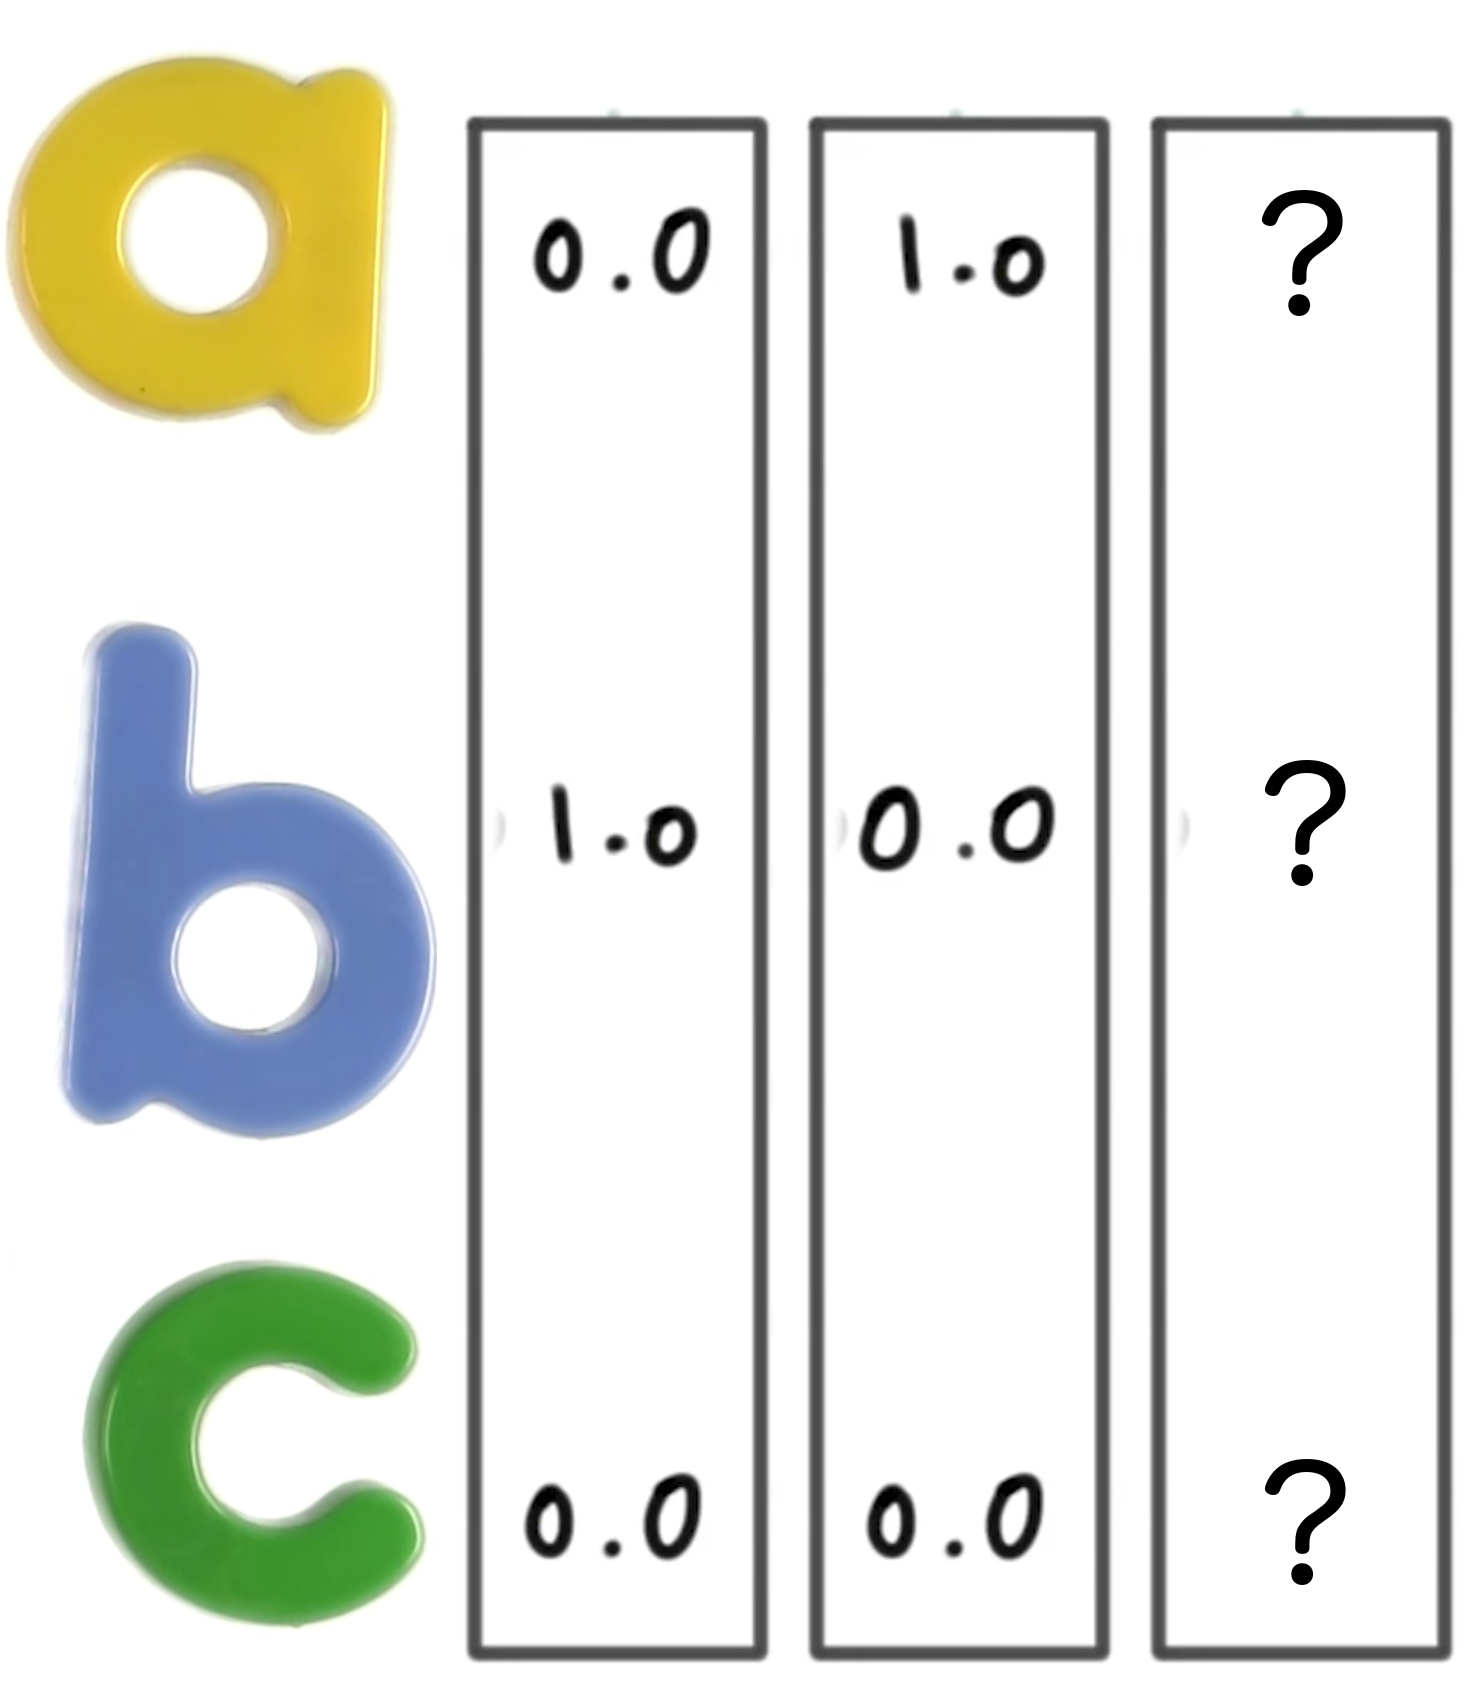
\includegraphics[width=0.5\linewidth]{./base-hot-enc}
%	\end{center}
%}



\frame{
\frametitle{Logistic classifier}
\begin{itemize}
\item Implemented by a neural network with multiple outputs (each output for each class).
\begin{equation}
\hat{Y} = f(XW + B)
\end{equation}
\item lets suppose a new "letter" image comes in.
\begin{center}
	
\includegraphics[trim={0 3cm 0 3cm},clip,height=0.15\textheight]{./b}
\end{center}
\pause
\item The output could be:
\begin{equation*}
	\hat{Y} = f(XW + B) = \begin{bmatrix}
	0.9  \\
	1.9  \\
	0.2  \\
	\end{bmatrix}
\end{equation*}
\item Such outputs ($\hat{y}$) are called logits

\end{itemize}
}


\frame{
\frametitle{Softmax function}
\framesubtitle{Distribution over classes}
\begin{itemize}
	\item We need to convert them into probabilities $p(x=c_i|z)$
	\begin{equation*}
		\hat{Y} = \begin{bmatrix}
			0.9  \\
			1.9  \\
			0.2  \\
		\end{bmatrix}
		\rightarrow
		\begin{bmatrix}
			p = 0.2 \\
			p = 0.7 \\
			p = 0.1 \\
		\end{bmatrix}
	\end{equation*}
\item Softmax converts a vector into ``probabilities''
\begin{equation}
	S(\hat{y}_i) = \dfrac{e^{\hat{y}_i}}{\sum_{j}e^{\hat{y}_j}}
\end{equation}

\pause
\item Then:

\begin{equation*}
S(\hat{Y}) = \begin{bmatrix}
0.9  \\
1.9  \\
0.2  \\
\end{bmatrix}
\rightarrow
\begin{bmatrix}
p = 0.2 \\
p = 0.7 \\
p = 0.1 \\
\end{bmatrix}
\end{equation*}
\end{itemize}
}


\begin{frame}
	\frametitle{The predicted class}
	\begin{itemize}
		\item The predicted class is the index with the highest probability:
		\begin{equation}
			Max(S) = \arg\max_i s_i | s_i \in S	
		\end{equation}
		\pause
		\item Example\footnote{Supposing an indexing by one}:
		$$S = \begin{bmatrix}
			p = 0.2 \\
			p = 0.7 \\
			p = 0.1 \\
		\end{bmatrix}$$
		$$Max(S) = 2$$
		Recall that the second class is 'B'
	\end{itemize}
\end{frame}



\section{Multinomial logistic classifier}


\frame{
	\frametitle{Multinomial Logistic Classification}
	Steps:
	\begin{enumerate}
		\item Given an input $X$, obtain the neural network outputs: $$\hat{Y} = f(XW+B)$$ where $\hat{Y}$ is the prediction vector
		\item Convert it into probabilities: $$S(\hat{y}_i) = \dfrac{e^{\hat{y}_i}}{\sum_{j}e^{\hat{y}_j}}$$ 
		\item Return the index with highest probability:
		$$
		Max(S) = \arg\max_i s_i | s_i \in S	
		$$
	\end{enumerate}
}


\frame{
\frametitle{Multinomial Logistic Classification}
\begin{figure}
	\centering
	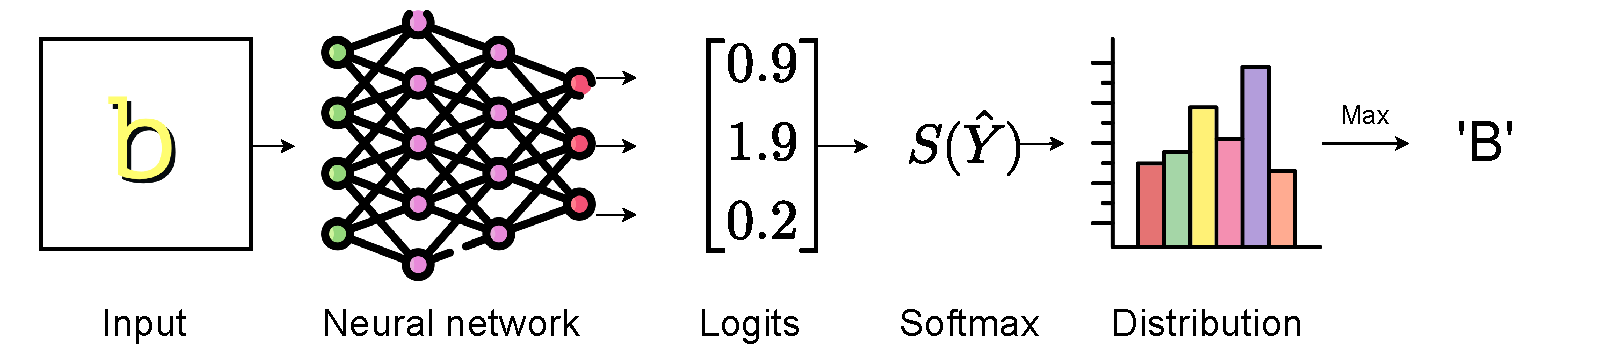
\includegraphics[height=0.4\textheight]{multinomial_notitle}
	\caption{Classification process}
	\label{fig:multinomial}
\end{figure}
}


\section{Data preprocessing}


% 1. Need for preprocessing

\begin{frame}
  \frametitle{Motivation}
  \begin{itemize}
    \item The scale and distribution of variables affects stability and speed of gradient descent.
    \item Poorly scaled data can saturate activations (e.g., sigmoid) and slow down learning.
    \item Adequate data prevents unbalanced gradients. \\
    \vspace{3mm}
      \textbf{Gradient descent:}
  $$
    \mathbf{W}^{(t+1)} \;=\; \mathbf{W}^{(t)} \;-\; \eta \,\nabla_{\mathbf{W}} \, L\!\big(\mathbf{W}^{(t)}\big)
  $$
  \small The magnitude of $\nabla L$ depends on the scale of inputs; rescaling/standardizing improves numerical conditioning.
  \end{itemize}
\end{frame}

% 2. Data transforms (overview)

\begin{frame}
  \frametitle{Data transforms: overview}
\vspace{3mm}
  
  
  \begin{itemize}
    \item Creating different “views” of the dataset can better reveal its structure.
    \item Two typical phases: \textit{fit} the parameters of the transform and \textit{apply} it.
    \item In neural networks, transformations support more stable optimization.
    \item Formally, 
  \begin{equation}
    \mathbf{x}' \;=\; T(\mathbf{x};\,\boldsymbol{\theta}), 
  \end{equation}
  $$
  \qquad 
    \boldsymbol{\theta} \leftarrow \operatorname{fit}(\mathcal{D})  
  $$
  \small Parameters $\boldsymbol{\theta}$ are estimated on training data, then $T$ is applied to train/validation/test sets.
  \end{itemize}
  
\end{frame}

% 3. Rescaling (Min–Max)
\begin{frame}
  \frametitle{Rescaling (Min--Max)}
  \begin{itemize}
    \item Homogenizes ranges (e.g., to $[0,1]$ or $[a,b]$).
    \item Useful for activation functions sensitive to magnitude and for training stability.
    \item Given a range $[a,b]$:
    \begin{equation}
        T_{\text{minmax}}(x_i;(a,b,X))
    \;=\;
    a \;+\;
    \frac{x_i - \min(X)}{\max(X) - \min(X)}\,(b-a)
    \end{equation} Common case: $a=0,\, b=1$. Fit only on training data to avoid data leakage.
  \end{itemize}
\end{frame}

\begin{frame}{Rescaling (Min-max)}
\framesubtitle{Example}
\begin{figure}
    \centering
    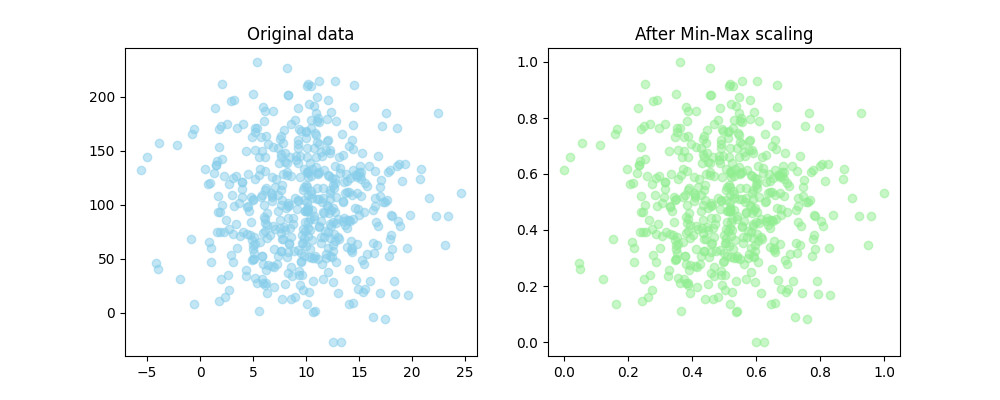
\includegraphics[width=0.9\linewidth]{min_max_multi.png}
    \caption{Rescaling keeps the distribution}
    \label{fig:placeholder}
\end{figure}
\end{frame}

% 4. Standardization (Z-score)

\begin{frame}
  \frametitle{Standardization (Z--score)}
  \begin{itemize}
    \item Centers and scales each variable to mean $0$ and standard deviation $1$.
    \item Balances weight updates and ensures well-conditioned gradients.
    \begin{equation}
        T_{\text{std}}(x_i; (\mu_i, \sigma_i))
    \;=\;
    \frac{x_i - \mu_i}{\sigma_i}
    \end{equation}
    $$
    \qquad\text{with}\quad
    \mu_i = \mathbb{E}[X],\;\;
    \sigma_i = \sqrt{\mathbb{V}[X]}    
    $$
    {\small Estimate $\mu_i,\sigma_i$ on training data and reuse them for validation/test.}
  \end{itemize}  
\end{frame}

\begin{frame}{Standardization}
\framesubtitle{Example}
    \begin{figure}
        \centering
        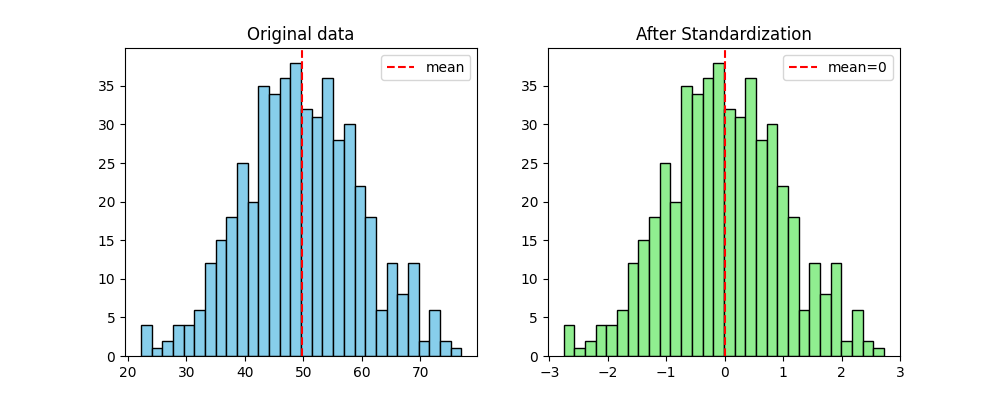
\includegraphics[width=0.9\linewidth]{histograms_standard.png}
        \caption{Data is adjusted to fit a zero centered distribution.}
        \label{fig:placeholder}
    \end{figure}
\end{frame}

% 5. Normalization by observation (unit norm)

\begin{frame}
  \frametitle{Normalization (unit norm)}
  \begin{itemize}
    \item Rescales each \emph{row} to have norm $1$ (typically L2).
    \item Useful when the direction of the vector matters more than its magnitude.
    \item Formally,
    \begin{equation}
        T_{\text{norm}}(\mathbf{x})
    =
    \frac{\mathbf{x}}{\lVert \mathbf{x}\rVert_2}
    \end{equation}
    \begin{equation}
        \lVert \mathbf{x}\rVert_2 \;=\; \sqrt{\sum_{j=1}^{d} x_j^2}        
    \end{equation}
    \item {\small Other norms (e.g., L1) can also be used depending on the problem.}
  \end{itemize}
\end{frame}

\begin{frame}{Normalization}
\framesubtitle{Example}
    \begin{figure}
        \centering
        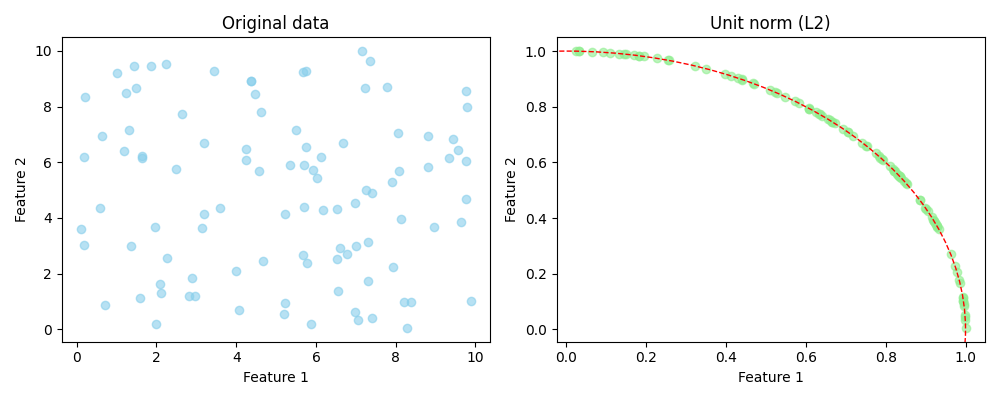
\includegraphics[width=0.9\linewidth]{unit_norm.png}
        \caption{In normalization the angles and differences are important}
        \label{fig:placeholder}
    \end{figure}
\end{frame}

% 6. Binarization (threshold)

\begin{frame}
  \frametitle{Binarization (threshold)}
  \begin{itemize}
    \item Converts continuous variables into binary ones based on a threshold $\tau$.
    \item Useful for feature engineering or discrete decision-making.
    \item Formally,
    \begin{equation}
    T_{\text{bin}}(x) = \mathbf{1}\{x > u\}
    \;=\;
    \begin{cases}
      1, & x > u\\[2pt]
      0, & x \le u
    \end{cases}    
    \end{equation}
    Threshold $u$ is chosen by domain knowledge or validation.
  \end{itemize}
\end{frame}

\frame{
   \frametitle{Binarization}
   \framesubtitle{Example}
   \begin{figure}
       \centering
       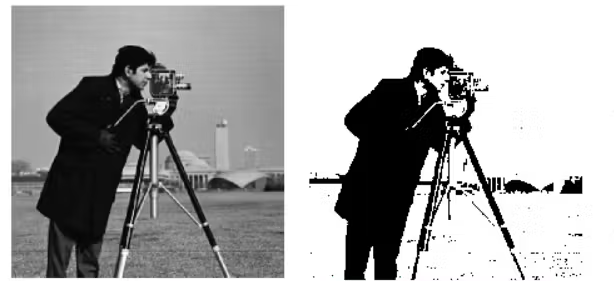
\includegraphics[width=0.8\linewidth]{otsu.png}
       \caption{Binarization of an image.}
       \label{fig:placeholder}
   \end{figure}
}

\frame{
	\frametitle{One-hot encoding}
	\framesubtitle{Target labels preprocessing}
	\begin{itemize}
		\item Facilitates the representation of categories in neural networks
		\item They are used to train the network
		\item Lets suppose the input image:
		\begin{center}
			
\includegraphics[height=0.15\textheight]{./a}
		\end{center}
		\item Then its label 'A' is converted
		\begin{equation*}
			L('A') = \begin{bmatrix}
				1.0 \\
				0.0 \\
				0.0 \\
			\end{bmatrix}
		\end{equation*}
	\end{itemize}
}

\frame{
	\frametitle{Categorical Data}
    \framesubtitle{One-hot encoding for features example}
	\begin{itemize}
		\item Admissions (again..). This dataset has three input features: GRE score, GPA, and the rank of the undergraduate school (numbered 1 through 4). Institutions with rank 1 have the highest prestige, those with rank 4 have the lowest.
		\begin{center}
			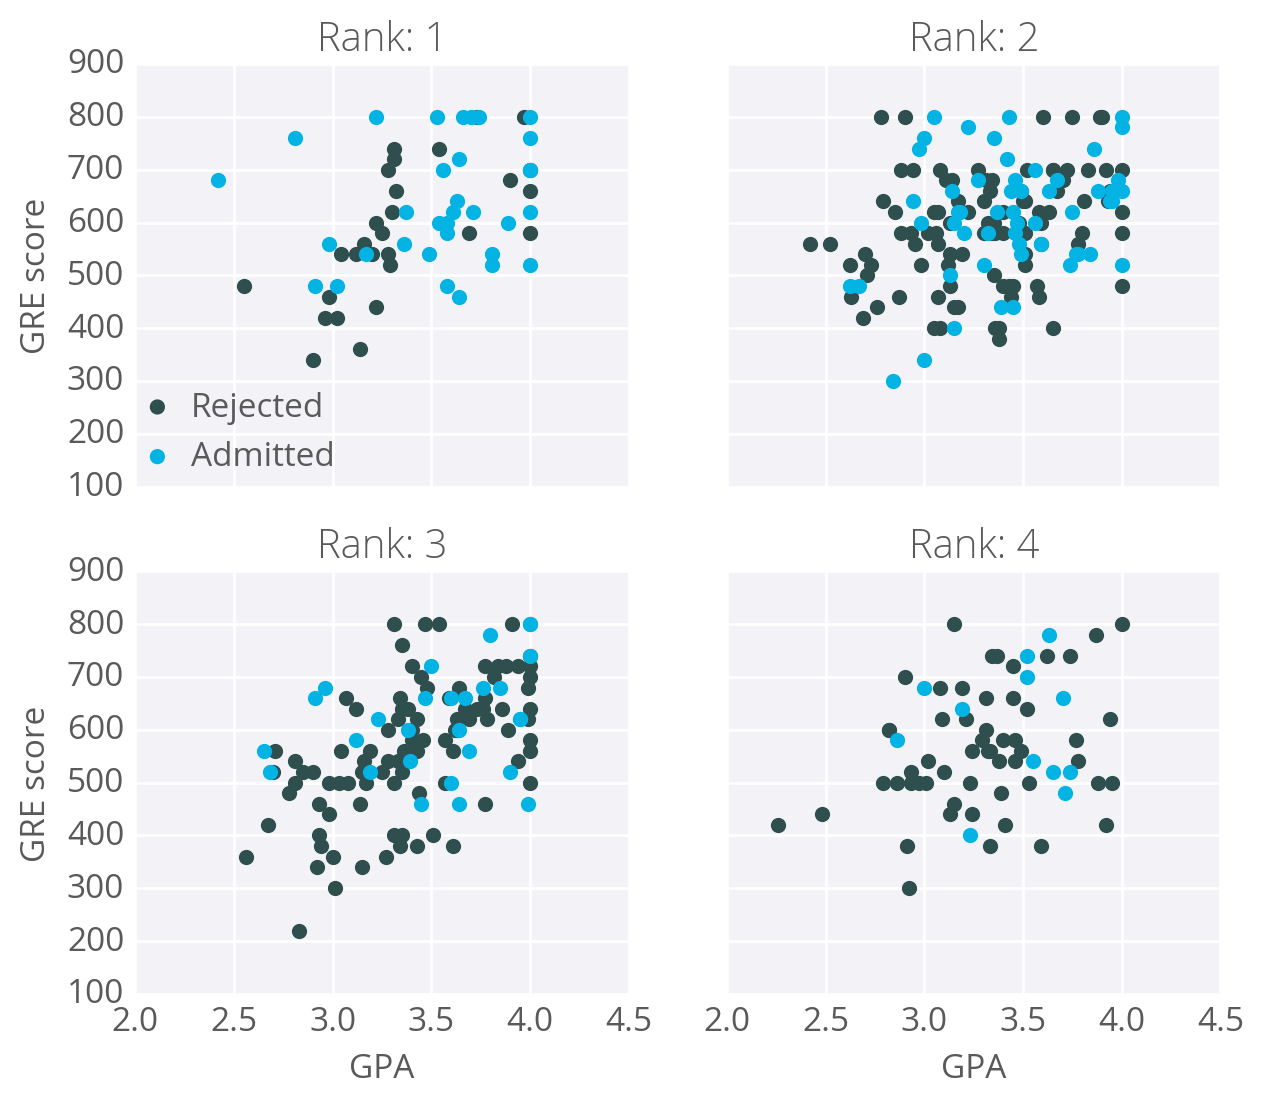
\includegraphics[height=0.6\textheight]{./admissions-data}
		\end{center}
	\end{itemize}
}


\frame{
	\frametitle{Categorical Data}
	\framesubtitle{One-hot encoding for features}
	\begin{itemize}
		\item Numerical and categorical data
		\item Add dummy variables.
		\begin{center}
			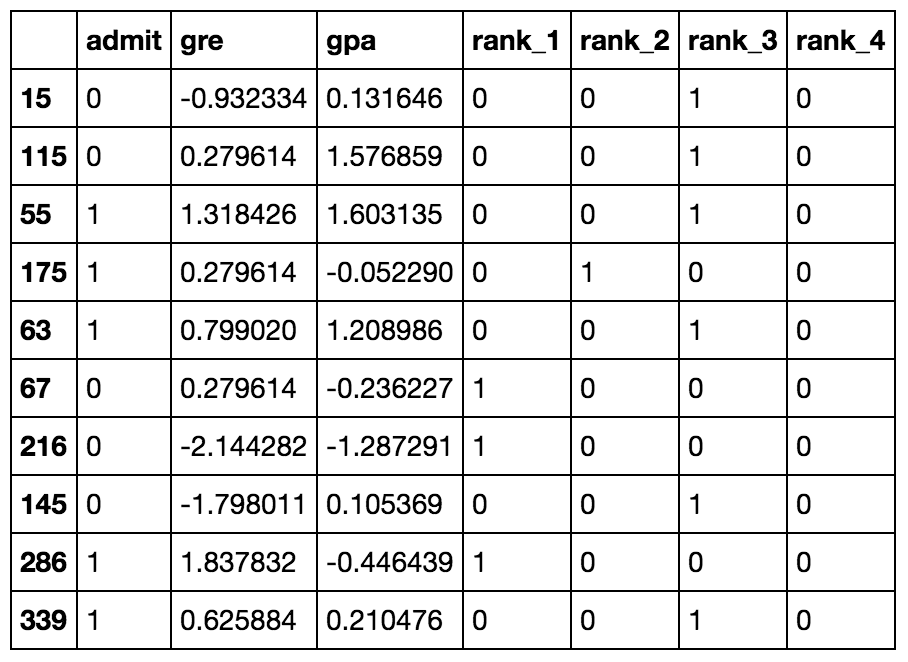
\includegraphics[height=0.6\textheight]{./example-data}
		\end{center}
	\end{itemize}
}



\section{Training}



\frame{
\frametitle{Multinomial Logistic Classification (2)}
\begin{itemize}
\item Multinomial Logistic classifier 
$$S(f(XW+B))$$
\pause
\item Do we hit?
\begin{figure}
	\centering
	
\includegraphics[height=0.4\textheight]{41guge}
	%\caption{}
	%\label{fig:41guge}
\end{figure}

\item To get the loss or error we measure the distance with respect to one-hot target vectors
$$D(S,L)$$
\end{itemize}

}


\frame{
	\frametitle{Cross Entropy}
	\framesubtitle{Loss function}
	\begin{itemize}
		\item Measures the distance between two probability vectors
		\begin{equation}
			D(S,L) = - \sum_{i} l_i \log (s_i)
		\end{equation} where $L$ is the target label.
		\item Substitution
			$$D(S(f(XW+B)),L)$$
		\item $D(S,L) \neq D(L,S)$
	\end{itemize}
}


\frame{
	\frametitle{Binary Cross Entropy}
	\framesubtitle{Loss function}
	\begin{itemize}
		\item Measures the distance
		\begin{equation}
			L(y, p) = -\frac{1}{N}\sum_{i=1}^{N} \left[ y_i \log(p_i) + (1 - y_i) \log(1 - p_i) \right]
		\end{equation} where $L$ is the target label.
		\item $L(y,p)$ is the binary cross entropy loss.
		\item $N$ is the number of samples.
		\item $y_i$ is the actual label of the $i^{th}$  sample
		\item $p_i$ is the predicted probability of the sample being in the positive class.
	\end{itemize}
}


\frame{
\frametitle{Training the Neural Network}
\begin{itemize}
\item Multinomial Logistic classifier
$$D(S(f(XW+B)),L)$$
\pause
\item What do we need to do?
\pause
\item Decrease the distances
$$\downarrow D(A,a)$$
$$\uparrow D(A,\neg a)$$
\pause
\item Loss = average cross entropy
\begin{equation}
	\mathcal{L}  = \frac{1}{N} \sum_{i} D(S(f(W x_i+B)),L_i)
\end{equation}
\end{itemize}
}


\frame{
	\frametitle{Minimizing the cross entropy}
\begin{figure}
	\centering
	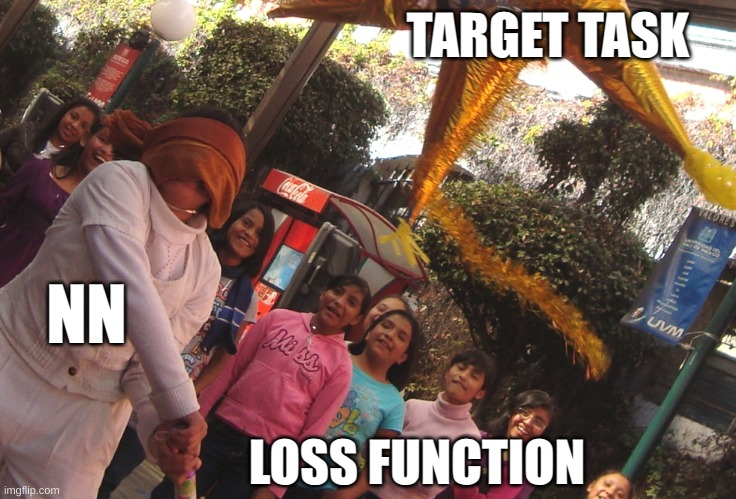
\includegraphics[height=0.7\textheight]{9o6bhy}
	\caption{Training with gradient descent}
	\label{fig:9o6bhy}
\end{figure}
}



\frame{
	\frametitle{Minimizing the cross entropy}
	\begin{itemize}
		\item The weights are updated with: $\Delta w$
	\end{itemize}
	
	\begin{figure}
		\centering
		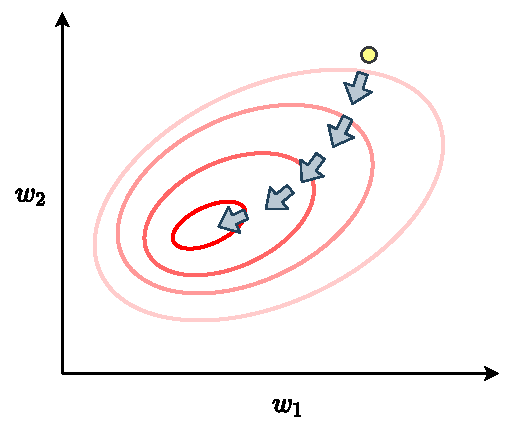
\includegraphics[height=0.7\textheight]{./gradient_descent}
		\caption{Gradient descent for $\mathcal{L}(w_1,w_2)$.}
		\label{fig:gradientdescent}
	\end{figure}
}


\frame{
	\frametitle{Training workflow}
\begin{figure}
	\centering
	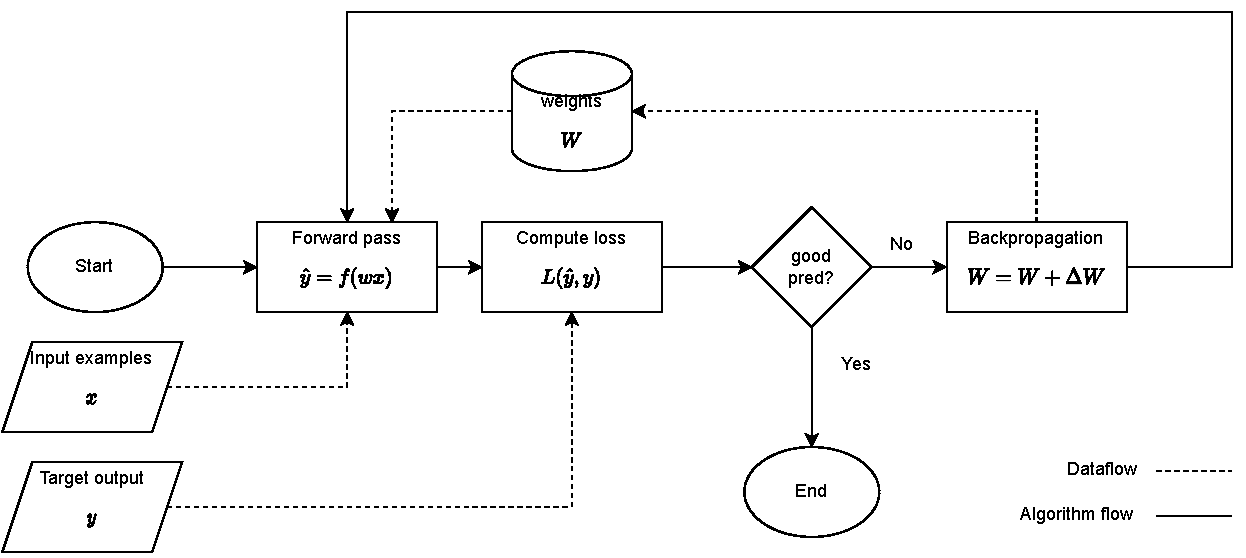
\includegraphics[height=0.7\textheight]{training_partial.drawio}
	\caption{Neural network training by gradient descent}
	\label{fig:trainingpartial}
\end{figure}
}

%\frame{
%\frametitle{Performance metrics}
%\begin{itemize}
%	\item Loss functions might not easy to understand or to analize the outputs.
%	\item Common measurements for categorical outputs:
%	\begin{description}
%		\item [Accuracy] $$Acc(\hat{f}) = \frac{1}{T} \sum_{i=1}^{T} (1_{y_i=\hat{y}_i})$$
%		\item [Accuracy error] 0-1 Loss
%		$$AccError(\hat{f}) = \frac{1}{T} \sum_{i=1}^{T} (1_{y_i\neq\hat{y}_i})$$
%	\end{description}
%\end{itemize}
%}



%\frame{
%\frametitle{Performance measurement}
%\framesubtitle{Cross validation}
%\begin{itemize}
%\item How do we split the observations?
%\end{itemize}
%
%\begin{description}
%\item [n-fold Cross validation] We could decide to split the observations into
%$n$ equally sized subsets.
%$$X_1,\dots,X_n$$ and use them as validation sets while the remainder is used to train the model.
%\end{description}
%\begin{itemize}
%\item Tipically $n=10$. This is \textit{10-fold cross validation}.
%\end{itemize}
%}


%
%\frame{
%\frametitle{Overfitting}
%\begin{center}
%\includegraphics[width=0.9\linewidth]{./validation}
%\end{center}
%}







%
%
%\frame{
%	\frametitle{}
%	\begin{itemize}
%		\item We will use TensorFlow to classify images from the notMNIST dataset 
%	\end{itemize}
%	
%	\begin{figure}
%		\centering
%		
\includegraphics[width=0.7\linewidth]{nmn.png}
%		\caption{}
%		\label{fig:nmn}
%	\end{figure}
%}
%
%\begin{frame}[fragile]
%\frametitle{Installation with anaconda}
%\begin{itemize}
%	\item 
%	Run the following commands to setup your environment:
%	{\small \begin{verbatim}
%		conda create --name=IntroToTensorFlow python=3 anaconda
%		source activate IntroToTensorFlow
%		conda install -c conda-forge tensorflow	
%		\end{verbatim}}
%	
%	\item That's it! 
%\end{itemize}	
%\end{frame}
%
%
%
%\begin{frame}[fragile]
%\frametitle{Hello World}
%\begin{verbatim}
%import tensorflow as tf
%
%# Create TensorFlow object called tensor
%hello_constant = tf.constant('Hello World!')
%
%with tf.Session() as sess:
%# Run the tf.constant operation in the session
%output = sess.run(hello_constant)
%print(output)
%\end{verbatim}
%\end{frame}
%
%
%\begin{frame}[fragile]
%\frametitle{Hello World}
%\begin{itemize}
%\item Tensor. It storages the values. Data is not stored as integers, floats, or strings. 
%\begin{verbatim}
%hello_constant = tf.constant('Hello World!')
%\end{verbatim}
%hello\_constant is a 0-dimensional string tensor	
%\item Examples
%\begin{verbatim}
%# A is a 0-dimensional int32 tensor
%A = tf.constant(1234) 
%# B is a 1-dimensional int32 tensor
%B = tf.constant([123,456,789]) 
%# C is a 2-dimensional int32 tensor
%C = tf.constant([ [123,456,789], [222,333,444] ])
%\end{verbatim}
%\end{itemize}
%\end{frame}
%
%
%\begin{frame}[fragile]
%\frametitle{Session}
%\begin{itemize}
%\item TensorFlow’s api is built around the idea of a computational graph
%
%\begin{center}
%\includegraphics[width=0.7\linewidth]{session.png}
%\end{center}
%\item A "TensorFlow Session", as shown above, is an environment for running a graph.
%\end{itemize}
%\end{frame}
%
%
%\begin{frame}[fragile]
%\frametitle{Exercises}
%\begin{itemize}
%\item Repositorio
%\url{https://github.com/irvingvasquez/cv2course_04tf}
%\item Exercises 01 and 02
%\end{itemize}	
%\end{frame}
%
%
%\begin{frame}[fragile]
%\frametitle{Mini project}
%
%Clone the Repository and Run the Notebook Run the commands below to clone the Lab Repository and then run the notebook:
%
%\url{https://github.com/irvingvasquez/CarND-TensorFlow-Lab}
%
%3 problems for you to solve:
%
%\begin{enumerate}
%\item Normalize the features
%\item Use TensorFlow operations to create features, labels, weight, and biases tensors
%\item Tune the learning rate, number of steps, and batch size for the best accuracy
%\end{enumerate}
%
%Make a report with your accuracy and parameters you use.
%\end{frame}


%\frame{
%\frametitle{Alternative project}
%\includegraphics[width=0.9\linewidth]{./cactus_0163.jpg}
%}


\begin{frame}
\frametitle{Lectures}
\begin{itemize}
	\item Jorge Luis Borges. Funes el memorioso.
\end{itemize}
\end{frame}


\frame{
\frametitle{References}
\centering

\includegraphics[width=0.2\textwidth]{mlm.png}

\includegraphics[width=0.2\textwidth]{norm.png}
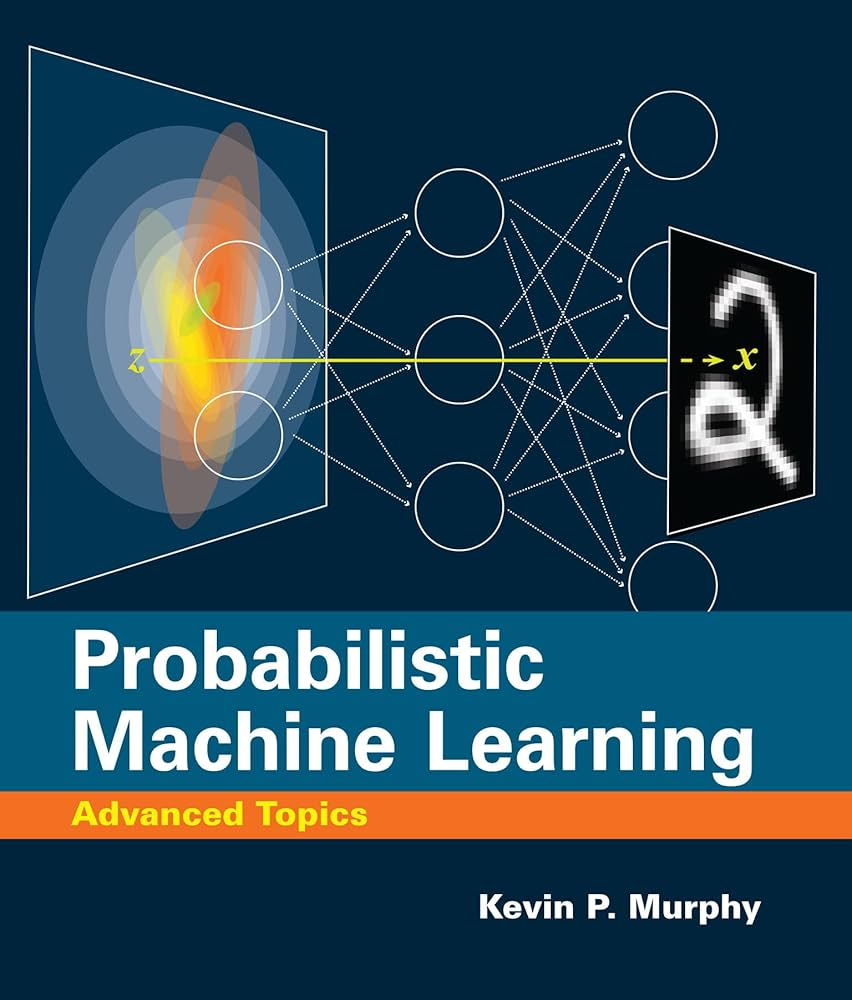
\includegraphics[width=0.2\textwidth]{pml.jpg}
}


\end{document}